\chapter{Anhang}
\label{ch:anhang}

\section{Implementierung}
\label{sec:anhang-implementierung}

\begin{figure}[htb]
	\centering
	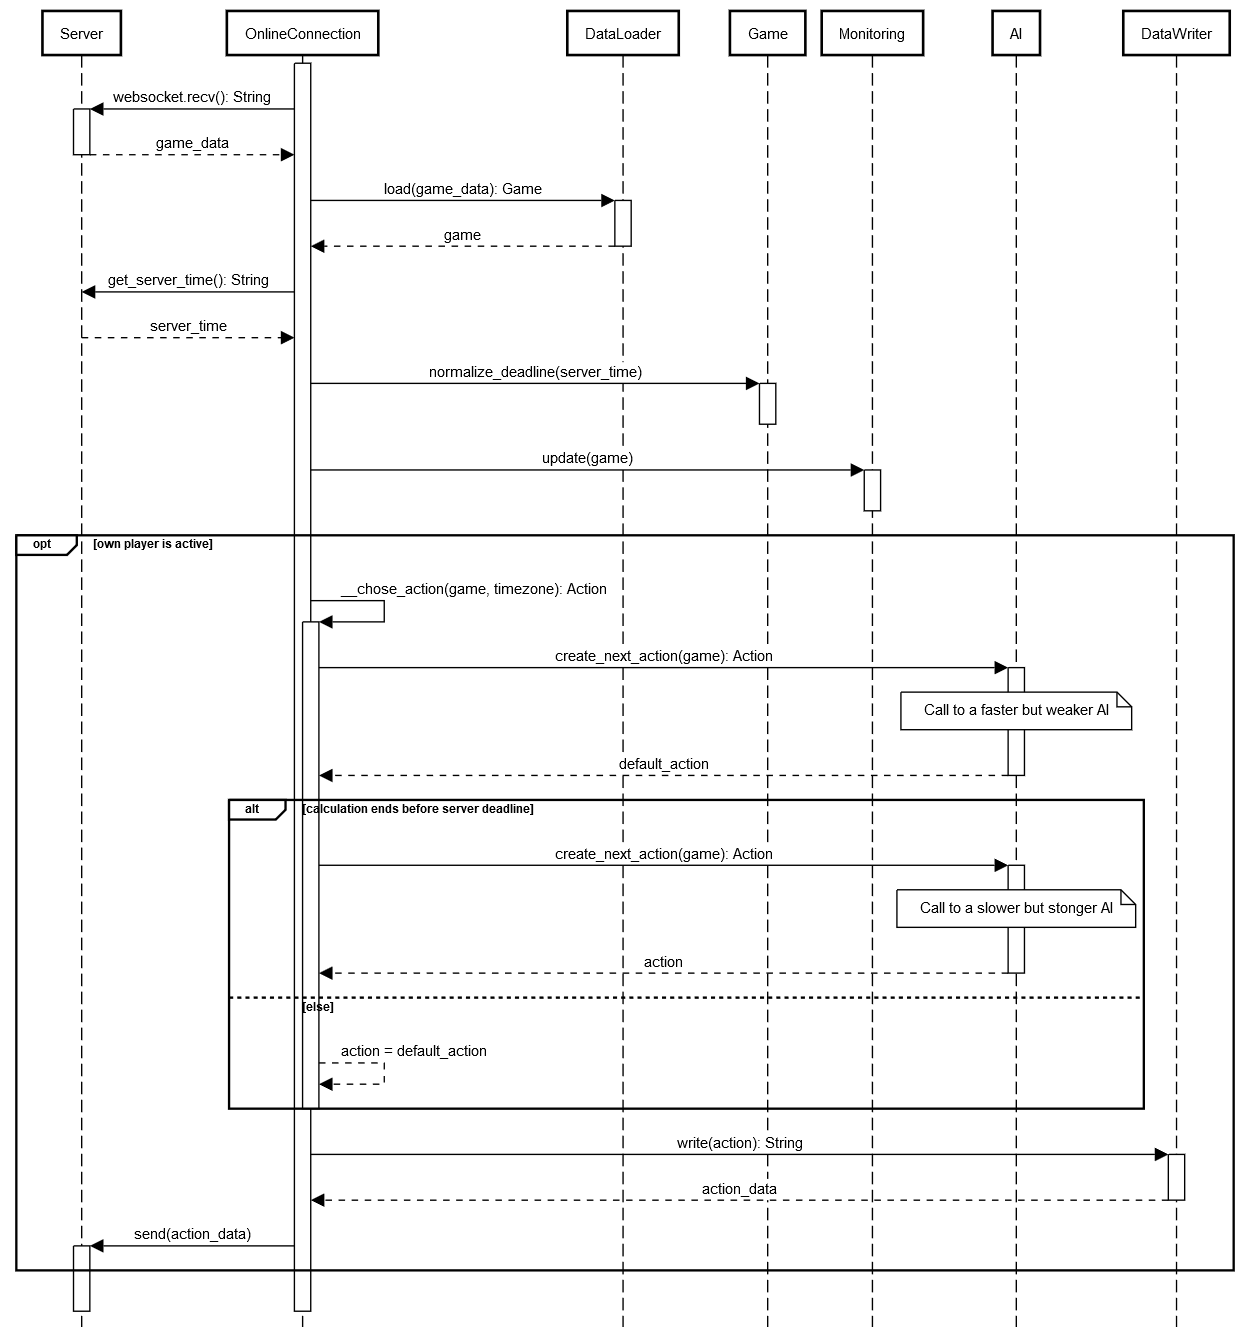
\includegraphics[width=13.5cm]{Bilder/Sequenzdiagramm_Implementierung_Spielzug.png}
	\caption{Sequenzdiagramm zur Implementierung eines Spielzug}
	\label{fig:sequenzdiagramm-spielzug}
\end{figure}

\begin{minipage}{\textwidth}
	\lstinputlisting[label=lst:json-spiel,language=JSON,caption=JSON-Repräsentation eines Spiel-Zustands]
	{../tests/test_data/ai/game_2.json}
\end{minipage}

\begin{minipage}{\textwidth}
	\lstinputlisting[label=lst:get-and-visit-cells
	,language=Python,caption=\Code{get\_and\_visit\_cells(player, action)}-Methode des \Code{GameService}]
	{./Dokumente/Get_And_Visit_Cells_GameService.txt}
	\lstinputlisting[label=lst:online-__play,language=Python,caption=\Code{\_\_play()}-Methode der \Code{OnlineConnection}]
	{./Dokumente/OnlineConnection-__play.txt}
\end{minipage}